\documentclass[
%   draft,
  a4paper,
%   titlepage,
  onecolumn,
%  twocolumn,
  11pt,
  ]%
% {scrartcl}%
{article}%


\usepackage[utf8x]{inputenc} 
%\usepackage[utf8]{inputenc} % codificação deste ficheiro em UTF-8 

\usepackage[T1]{fontenc} % necessário para que os caracteres acentuados possam ser considerados como um só bloco ( efeito colaterar: necessita de uma fonte que não a CM para não ficar com um aspecto aceitável)

%% precisa ser carregado um outro tipo de letra por causa do efeito colateral do pacote T1:
\usepackage{lmodern} % Fonte "Latin Modern" - A solução óptima para fontes latinas (resolve o problema do T1)
% \usepackage{times}   % Fonte "Times"


\usepackage{textcomp} % caracteres extra - símbolo do euro por exemplo

% \usepackage[portuguese]{babel} % tradução portuguesa
% \newcommand{\referencesname}{Bibliografia}
\newcommand{\referencesname}{References}


%%%%%%%%%% Packages


\usepackage[pdftex]{graphicx} % figuras 
% \usepackage{subfigure} % subfiguras ( a,b,... )
% \usepackage{wrapfig} % figuras ao lado de texto


\usepackage{array} % mais opções nas tabelas (m{width}, b{width}, ...)
\setlength{\extrarowheight}{1pt} % extra espaço entre as linhas das tabelas
% \usepackage{multirow} % tabelas com células multilinha

\usepackage{fancyhdr} % Estilo de página

% \usepackage{listings} % Highlight de código fonte
% \renewcommand{\lstlistingname}{Listagem} % tradução para português (referente ao package listings)
% \renewcommand{\lstlistlistingname}{Listagens} % tradução para português (referente ao package listings)

\usepackage[usenames,hyperref,pdftex%
 ,svgnames%
 ,x11names%
 ,dvipsnames%
%  ,cmyk
 ]{xcolor} % Utilização de cores
\usepackage{multicol}


\usepackage[left=2.3cm,right=2.3cm,top=2.4cm]{geometry} % Margins

% \usepackage{setspace} % spacing between lines (\singlespacing, \onehalfspacing, ...)

% math packages by AMS
\usepackage{amsmath} % main one
% \usepackage{amsfonts}
% \usepackage{amssymb}


% \usepackage{moreverb} % more verbatim options (boxedverbatim)
\usepackage{fancyvrb} % more verbatim options 

% \usepackage{lipsum}


% \usepackage{tikz}
% Optional tikz libraries
% \usetikzlibrary{arrows}


\usepackage[square, comma, sort&compress]{natbib}

\setcitestyle{super,comma}

% \usepackage[protrusion=true,expansion=true]{microtype}
\usepackage[protrusion=true,expansion=true,stretch=10,shrink=10]{microtype} % micro-typographic extensions of pdfTEX (gets high quality text compostion)

\usepackage[
      pdftex,             %driver
      colorlinks=true,    %no frame around URL
      urlcolor=DarkGreen!70!Black,    %no colors
%       menucolor=black,    %no colors
      linkcolor=black,    %no colors
%       pagecolor=black,    %no colors
      citecolor=DarkGreen!70!Black,    %no colors
      bookmarks=true,    %tree-like TOC
      bookmarksopen=true,    %expanded when starting
      bookmarksnumbered=true, %Put section numbers in bookmarks
      hyperfootnotes=true,    %no referencing of footnotes, does not compile
      pdfpagemode=UseOutlines,    %show the bookmarks when starting the pdf viewer
      plainpages=false, %solve problem ``destination with the same identifier'' warning
      pdfpagelabels %solve problem ``destination with the same identifier'' warning
]{hyperref} % fazer hyperlinks (usar como último ``usepackage'')


% \usepackage[style=altlist,hypertoc,hyper,number=page]{glossary}


% \usepackage{pdfpages}

 \usepackage[]{todonotes}
% \usepackage[disable]{todonotes}

\usepackage{xifthen}
\usepackage{csvsimple}



\newcommand{\tab}{\hspace*{2em}}

%Text subscript
\usepackage{fixltx2e}

% Matrizes
\usepackage{amsmath}

%rename defaults

\renewcommand{\figurename}{Figura}
\renewcommand{\contentsname}{Tabela de conteúdos}
\renewcommand{\abstractname}{Introdução}
\renewcommand{\refname}{Referências}


%Figure side by side

\usepackage{subfig}

%force float position
\usepackage{float}
\usepackage[section]{placeins}

\makeatletter
\AtBeginDocument{%
  \expandafter\renewcommand\expandafter\subsection\expandafter{%
    \expandafter\@fb@secFB\subsection
  }%
}
\makeatother
%%%%%%%%%%%%%%%%%%%%%%%%%%%%%%%%%%%%%%%%%%%%%%%%%%%%%%%%%%%%%%%% 


% Ifenização
%\hyphenation{apli-ca-ção cons-tru-ção}% ...

%%%%%%%%%%%%%%%%%%%%%%%%%%%%%%%%%%%%%%%%%%%%%%%%%%%%%%%%%%%%%%%%
%Parametros de exibicao de codigo
\usepackage{listings}
\usepackage{color}

\definecolor{mygreen}{rgb}{0,0.6,0}
\definecolor{mygray}{rgb}{0.5,0.5,0.5}
\definecolor{mymauve}{rgb}{0.58,0,0.82}

\lstset{ %
  backgroundcolor=\color{white},   % choose the background color; you must add \usepackage{color} or \usepackage{xcolor}
  basicstyle=\footnotesize,        % the size of the fonts that are used for the code
  breakatwhitespace=false,         % sets if automatic breaks should only happen at whitespace
  breaklines=true,                 % sets automatic line breaking
  captionpos=b,                    % sets the caption-position to bottom
  commentstyle=\color{mygreen},    % comment style
  deletekeywords={...},            % if you want to delete keywords from the given language
  escapeinside={\%*}{*)},          % if you want to add LaTeX within your code
  extendedchars=true,              % lets you use non-ASCII characters; for 8-bits encodings only, does not work with UTF-8
  frame=single,                    % adds a frame around the code
  keepspaces=true,                 % keeps spaces in text, useful for keeping indentation of code (possibly needs columns=flexible)
  keywordstyle=\color{blue},       % keyword style
  language=Matlab,                 % the language of the code
  morekeywords={*,...},            % if you want to add more keywords to the set
  numbers=left,                    % where to put the line-numbers; possible values are (none, left, right)
  numbersep=5pt,                   % how far the line-numbers are from the code
  numberstyle=\tiny\color{mygray}, % the style that is used for the line-numbers
  rulecolor=\color{black},         % if not set, the frame-color may be changed on line-breaks within not-black text (e.g. comments (green here))
  showspaces=false,                % show spaces everywhere adding particular underscores; it overrides 'showstringspaces'
  showstringspaces=false,          % underline spaces within strings only
  showtabs=false,                  % show tabs within strings adding particular underscores
  stepnumber=2,                    % the step between two line-numbers. If it's 1, each line will be numbered
  stringstyle=\color{mymauve},     % string literal style
  tabsize=2,                       % sets default tabsize to 2 spaces
  title=\lstname                   % show the filename of files included with \lstinputlisting; also try caption instead of title
  %inputencoding=ansinew
}


%%%%%%%%%%%%%%%%%%%%%%%%%%%%%%%%%%%%%%%%%%%%%%%%%%%%%%%%%%%%%%%%

%% Criação de comandos:


\newcommand{\note}[1]{{\sffamily \slshape \textcolor{red}{#1}}}

\colorlet{FPathColor}{Sepia}
\colorlet{CmdColor}{blue}
\colorlet{CmdRuleColor}{LightSteelBlue}
\colorlet{FileTextColor}{DarkGreen}
\colorlet{FuncColor}{DeepPink4}
\CustomVerbatimCommand{\FPath}{Verb}{formatcom=\color{FPathColor},fontsize=\normalsize}
\CustomVerbatimCommand{\Cmd}{Verb}{formatcom=\color{CmdColor},fontsize=\normalsize}
\CustomVerbatimCommand{\FText}{Verb}{formatcom=\color{FileTextColor},fontsize=\normalsize}
\CustomVerbatimCommand{\Func}{Verb}{formatcom=\color{FuncColor},fontsize=\normalsize}
\DefineVerbatimEnvironment%
  {Command}{Verbatim}
  {formatcom=\color{CmdColor},frame=single,rulecolor=\color{CmdRuleColor},fontsize=\normalsize}
\DefineVerbatimEnvironment%
  {FileText}{Verbatim}
  {formatcom=\color{FileTextColor},fontsize=\normalsize}


% % Authors:



\newcommand{\MYauthor}{José Pedro Medeiros}
\newcommand{\MYnumber}{2010129934} 

\newcommand{\MYauthorII}{Luís Miguel Rocha} 
\newcommand{\MYnumberII}{2010127532}

%\newcommand{\MYauthorIII}{------ ----- ----} 
%\newcommand{\MYnumberIII}{xxxxxxxxxx}



% % Titles:
\newcommand{\MYtitle}{Estimação de Movimento (Cálculo do Fluxo Óptico)}
\newcommand{\MYsubtitle}{Trabalho Prático nº4} % Can be empty


% % Course

\newcommand{\MYcoursename}{Visão por Computador}
\newcommand{\MYcourseyear}{2013/2014}


% % PDF infos

\newcommand{\MYkeywords}{} % Can be empty
\newcommand{\MYsubject}{} % Can be empty


%% Document format

%% Fancy Headers
\lhead{
\includegraphics[width=2cm]{logo_deec.pdf}}
\chead{\sc\footnotesize Universidade de Coimbra\\
Faculdade de Ciências e Tecnologia\\
Departamento de Engenharia Electrotécnica e de Computadores}
\rhead{
\includegraphics[width=0.8cm]{logo_fctuc.pdf}}
\setlength{\headheight}{43pt}

% Title
\title{{\large\MYcoursename\ -- \MYcourseyear}\\[2mm]
{\MYtitle}
\ifthenelse{\equal{\MYsubtitle}{}}
{\vspace*{1mm}}   {\\{\large\MYsubtitle}\vspace*{1mm}}
}

% Author / Number
\author{%
\MYauthor\\{\normalsize \href{mailto:ze_pedrom@hotmail.com}{\MYnumber}}
\ifthenelse{\isnamedefined{MYauthorII}}
{\and\MYauthorII\\{\normalsize \href{mailto:luis.rocha.jacinto@gmail.com}{\MYnumberII}}}    {}
\ifthenelse{\isnamedefined{MYauthorIII}}
{\and\MYauthorIII\\{\normalsize \href{mailto:a\MYnumberIII@alunos.deec.uc.pt}{\MYnumberIII}}}   {}
}

% Version / Date
\date{%
% \normalsize \today
\mbox{}
}




%% PDF definitions:

\hypersetup{%
   pdftitle=\MYtitle,%
   pdfauthor=\MYauthor,%
%    pdfcreator=,%
   pdfkeywords= {\MYkeywords},%
%    pdfproducer=,%
   pdfsubject= \MYsubject%
} % informações do pdf (pacote hyperref)

\pdfinfo{
/Title	(\MYtitle)
/Author (\MYauthor)
/Keywords (\MYkeywords)
} % informações do pdf

\graphicspath{ {img/} } % Pasta das Imagens










\begin{document}

\maketitle
\thispagestyle{fancyplain}

\setlength{\parskip}{10pt}
% Introdução
 \begin{abstract} % (optional)
 
 Neste trabalho foram calculadas as componentes de movimento de uma sequência de imagens, ou seja, o fluxo óptico. Estes cálculos foram feitos para dois tipos de modelos, o modelo constante para o movimento e o modelo afim para o movimento. Posteriormente calcularam-se os vectores médios de movimento que são comparados com o movimento original imposto. Por fim os passos anteriores foram repetidos para diferentes movimentos e para diferentes deslocamentos.
 
 
 \end{abstract}



\begin{figure}[ht]
\centering
\includegraphics[width=70mm,scale=0.5]{img.png}
\caption{Imagem original}\label{fig:img}
\end{figure}



\newpage

% Indice
%\newpage
 \tableofcontents

%Inicio
\newpage



\section{Cálculo do Fluxo Óptico}

Para o cálculo das derivadas parciais usamos as seguintes fórmulas:
\setlength{\parskip}{10pt}

$I_x{(x,y)}= [(-I_1{(x,y)} - I_1{(x,y+1)} + I_1{(x+1,y)} + I_1{(x+1,y+1)}) + (-I_2{(x,y)} - I_2{(x,y+1)} + I_2{(x+1,y)} + I_2{(x+1,y+1)})]/4;$
\setlength{\parskip}{7pt}

$I_y{(x,y)} = [(-I_1{(x,y)} - I_1{(x+1,y)} + I_1{(x,y+1)} + I_1{(x+1,y+1)}) + (-I_2{(x,y)} - I_2{(x+1,y)} + I_2{(x,y+1)} + I_2{(x+1,y+1)})]/4;$
\setlength{\parskip}{7pt}

$I_t{(x,y)} = [(-I_1{(x,y)} - I_1{(x,y+1)} - I_1{(x+1,y)} - I_1{(x+1,y+1)}) + (I_2{(x,y)} + I_2{(x,y+1)} + I_2{(x+1,y)} + I_2{(x+1,y+1)})]/4;$ 

\setlength{\parskip}{15pt}


\textbf{Modelo Constante}


\begin{equation}\label{eq:1}
%
    \begin{bmatrix}
I\textsubscript{x\textsubscript{1}} & I\textsubscript{y\textsubscript{1}} \\
I\textsubscript{x\textsubscript{2}} & I\textsubscript{y\textsubscript{2}} \\
\vdots & \vdots \\
I\textsubscript{x\textsubscript{n}} & I\textsubscript{y\textsubscript{n}} 
 \end{bmatrix} 
 =
  \begin{bmatrix}
  a_x \\ a_y
    \end{bmatrix}
     \times
    \begin{bmatrix}
        -I\textsubscript{t\textsubscript{1}} \\
 -I\textsubscript{t\textsubscript{2}}\\
 \vdots \\
  -I\textsubscript{t\textsubscript{n}}
    \end{bmatrix}
%
\end{equation}

, onde V\textsubscript{x} = a\textsubscript{x} = constante  e V\textsubscript{y} = a\textsubscript{y} = constante. 

\setlength{\parskip}{7pt}




\textbf{Modelo Afim}





\begin{equation}\label{eq:2}
%
    \begin{bmatrix}
I\textsubscript{x\textsubscript{1}} & I\textsubscript{x\textsubscript{1}} x & I\textsubscript{x\textsubscript{1}} y & I\textsubscript{y\textsubscript{1}} & I\textsubscript{y\textsubscript{1}}\times x & I\textsubscript{y\textsubscript{1}}y \\
I\textsubscript{x\textsubscript{2}} & I\textsubscript{x\textsubscript{2}} x & I\textsubscript{x\textsubscript{2}} y & I\textsubscript{y\textsubscript{2}} & I\textsubscript{y\textsubscript{2}}\times x & I\textsubscript{y\textsubscript{2}} y \\
\vdots & \vdots & \vdots & \vdots & \vdots & \vdots \\
I\textsubscript{x\textsubscript{n}} & I\textsubscript{x\textsubscript{n}} x & I\textsubscript{x\textsubscript{n}} y & I\textsubscript{y\textsubscript{n}} & I\textsubscript{y\textsubscript{n}}\times x & I\textsubscript{y\textsubscript{n}} y \\
 \end{bmatrix} 
 =
  \begin{bmatrix}
  a_0 \\
   a_1 \\
   a_2 \\
   b_0 \\
   b_1 \\
   b_2	\\
   
    \end{bmatrix}
     \times
    \begin{bmatrix}
        -I\textsubscript{t\textsubscript{1}} \\
 -I\textsubscript{t\textsubscript{2}}\\
 \vdots \\
  -I\textsubscript{t\textsubscript{n}}
    \end{bmatrix}
%
\end{equation}

, onde V\textsubscript{x} = a\textsubscript{0} + a\textsubscript{1}x + a\textsubscript{2}y  e V\textsubscript{y} = b\textsubscript{0} + b\textsubscript{1}x + b\textsubscript{2}y.



\textbf{Nota}: Para obtermos os coeficientes $\begin{bmatrix}  a_x \\ a_y    \end{bmatrix}$ e   $\begin{bmatrix}   a_0 \\ a_1 \\ a_2 \\ b_0 \\ b_1 \\ b_2	\\ \end{bmatrix}$ fazemos uso da pseudo-inversa nas equações \eqref{eq:1} e \eqref{eq:2} usando o método dos minimos quadrados.



\newpage

\section{Trabalho Práctico}

\subsection{Movimento de 1 Pixel}

\subsubsection{Modelo Constante - Janela 5x5}



\begin{figure}[ht]
\centering
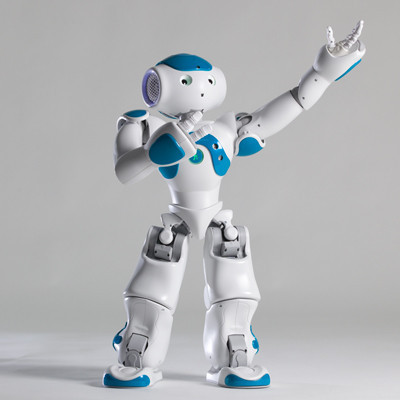
\includegraphics[width=140mm,scale=0.5]{1.jpg}
\caption{Janela de 5x5 - Deslocação de 1 Pixel}\label{fig:1}
\end{figure}



Na figura \ref{fig:1} efectuamos um movimento de 1 pixel em todas as imagens \textbf{excepto} na primeira. Decidimos usar uma janela de 5x5 para o calculo do fluxo óptico e usamos um espaçamento de 20 pixeis para a marcação do vector de movimento que sobrepusemos com as respectivas imagens. Na imagem do canto superior esquerdo verificamos que o vector de movimento é nulo, o que condiz com o pressuposto visto que para o calculo do fluxo óptico usamos a mesma imagem. Na imagem do canto superior direito vizualizamos um vector de movimento  sobreposto á imagem com a direção na diagonal. Isto deve-se ao facto de termos deslocado essa imagem na diagonal. Para o o calculo das derivadas parcias\footnote{Ver função \textbf{calcula\_Ix\_Iy\_It}}fizemos uso da matriz da imagem original e da imagem deslocada na diagonal. Nas duas imagens restantes repetimos o procedimento mas deslocamos os um pixel na horizontal e na vertical respectivamente.

\newpage

Calculamos as componentes das velocidades respectivas para cada movimento, sendo estas:





 \begin{multicols}{2}

\begin{enumerate}
  \item Nenhum Movimento
 
  \begin{enumerate}
    \item Vx = 0
    \item Vy = 0
    \item $\sigma_{V_x} = 0 $
    \item $\sigma_{V_y} = 0 $
  \end{enumerate}
  \item Movimento na Horizontal
  \begin{enumerate}
    \item Vx = 0.7219
    \item $Vy \approx 0$
    \item $\sigma_{V_x} = 0.4494 $
    \item $\sigma_{V_y} = 0.0023 $ 
  \end{enumerate}
  \item Movimento na Vertical
  \begin{enumerate}
    \item Vx = 0.0030
    \item Vy = 0.7130
    \item $\sigma_{V_x} = 0.0385 $
    \item $\sigma_{V_y} = 0.4521 $ 
  \end{enumerate}
  \item Movimento na Diagonal
  \begin{enumerate}
   \item Vx = 0.6330
    \item Vy = 0.6025
    \item $\sigma_{V_x} = 0.5398 $
    \item $\sigma_{V_y} = 0.5048 $ 
  \end{enumerate}
\end{enumerate}

\end{multicols}


\setlength{\parskip}{20pt}

Concluimos que a média da velocidade em x e em y condiz com o movimento que efectuamos para cada caso. Podemos comprovar isso analisando o valor da velocidade em x, $V_x$, e em y, $V_y$. Por exemplo, no movimento horizontal espera-se que o valor médio de $V_x$ tenha um valor próximo de 1 e o valor médio de $V_y$ tenha um valor próximo de 0 e de facto os valores que obtivemos para esse movimento condizem com o esperado tendo o $V_x$ o valor de 0.7219 e o $V_y$ o valor aproximadamente 0 . Os valores que obtivemos comprovam que o algoritmo calculou bem a média dos vectores de movimento. O cálculo do desvio de padrão (modulo e direcção) assim como a velocidade média de $V_x$ e $V_y$ podem ser vistos no nosso códico Matlab desenvolvido.\footnote{Ver função \textbf{modelo}}.



\newpage

\subsubsection{Modelo Afim - Janela 5x5}



\begin{figure}[ht]
\centering
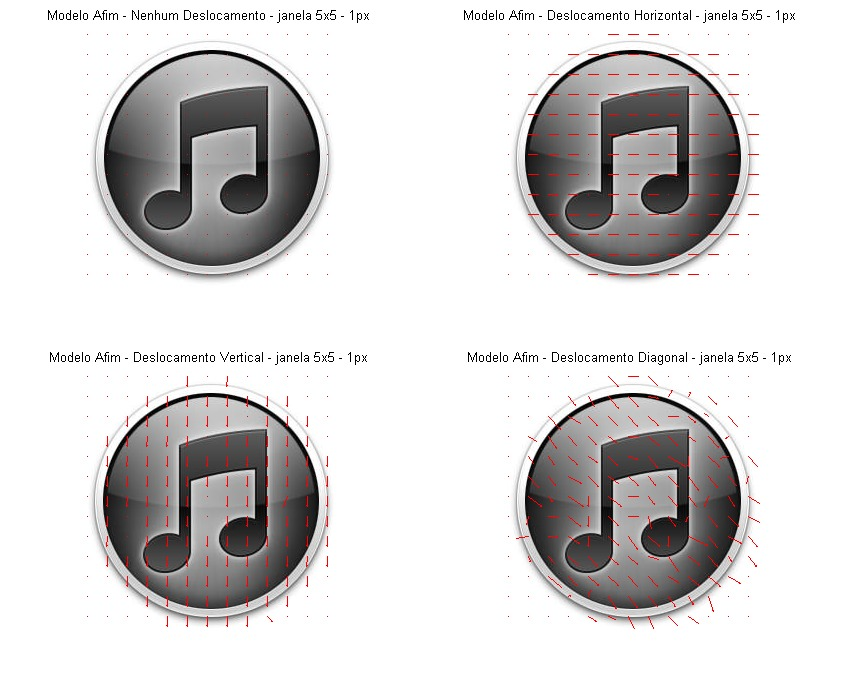
\includegraphics[width=140mm,scale=0.5]{2.jpg}
\caption{Janela de 5x5 - Deslocação de 1 Pixel}\label{fig:2}
\end{figure}


\setlength{\parskip}{20pt}
Na figura \ref{fig:2} voltamos a efectuar um movimento de 1 pixel em todas as imagens \textbf{excepto} na primeira. Neste caso usamos o modelo afim para o cálculo do fluxo óptico. Observando a imagem acima não se verifica uma grande diferença em termos do vector de velocidades sobreposto ás respectivas imagens. Em termos de comparação ambos os modelos detectam bem o movimento efectuado nos pixeis. Optamos por uma janela de 5x5 novamente para podermos comparar os resultados obtidos.

\newpage

Calculamos as componentes das velocidades respectivas para cada movimento, sendo estas:





 \begin{multicols}{2}

\begin{enumerate}
  \item Nenhum Movimento
 
  \begin{enumerate}
    \item Vx = 0
    \item Vy = 0
    \item $\sigma_{V_x} = 0 $
    \item $\sigma_{V_y} = 0 $
  \end{enumerate}
  \item Movimento na Horizontal
  \begin{enumerate}
    \item Vx = 0.7219
    \item $Vy \approx 0$
    \item $\sigma_{V_x} = 0.4494 $
    \item $\sigma_{V_y} = 0.0041 $ 
  \end{enumerate}
  \item Movimento na Vertical
  \begin{enumerate}
    \item Vx = 0.0011
    \item Vy = 0.7130
    \item $\sigma_{V_x} = 0.0455 $
    \item $\sigma_{V_y} = 0.4521 $ 
  \end{enumerate}
  \item Movimento na Diagonal
  \begin{enumerate}
   \item Vx = 0.6311
    \item Vy = 0.6030
    \item $\sigma_{V_x} = 0.5425 $
    \item $\sigma_{V_y} = 0.5042 $ 
  \end{enumerate}
\end{enumerate}

\end{multicols}




Analisando os valores de $V_x$ e $V_y$ concluimos, tal como no modelo constante, que o modelo afim está a calcular bem os vectores de velocidade. Comparando os valores de $V_x$ e $V_y$ do Modelo Afim com os do Modelo Constante podemos constatar que os valores são muito semelhantes. Essa mesma conclusão pode ser retirada analisando os vectores de velocidade marcados na \ref{fig:1} e \ref{fig:2} que são muito idênticos.




\newpage

\subsection{Movimento de 5 Pixeis}

\subsubsection{Modelo Constante - Janela 8x8}



\begin{figure}[ht]
\centering
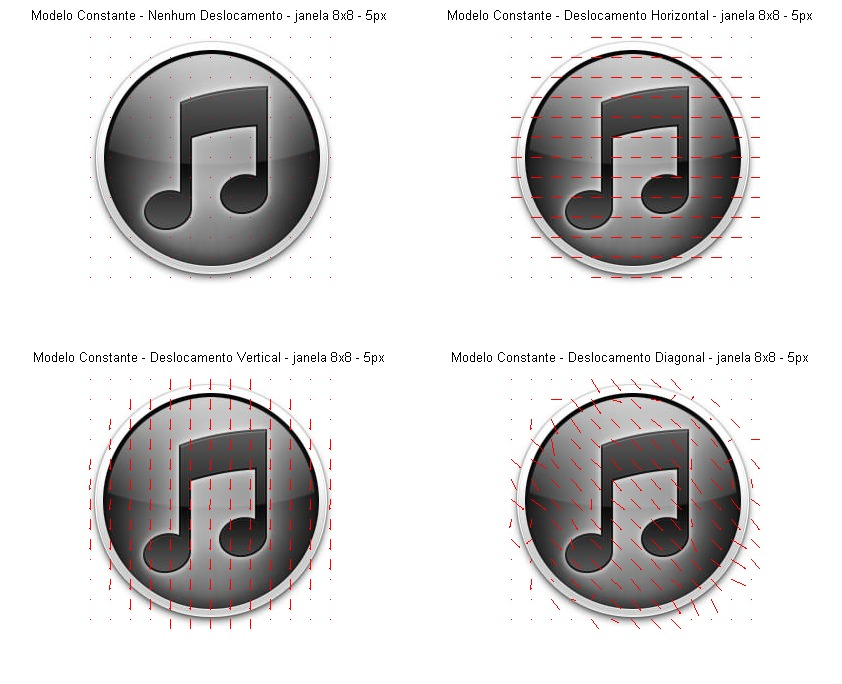
\includegraphics[width=140mm,scale=0.5]{3.jpg}
\caption{Janela de 8x8 - Deslocação de 5 Pixel}\label{fig:3}
\end{figure}

\setlength{\parskip}{20pt}

Na figura \ref{fig:3} estão representados os vectores de movimentos calculados com uma janela 8x8. Cada imagem sofreu um desclocamento de 5 pixeis exceptuando a do canto superior esquerdo. Observando a direcção dos vectores de velocidade verificamos que correspondem ás direcções das movimentações dos pixeis. Comparando a figura \ref{fig:1} com a figura \ref{fig:3} podemos ver que não se detecta muitas diferenças em termos dos vectores de velocidade, no entanto, verificamos através dos valores vistos no \textit{Matlab} que o desvio de padrão é menor, ou seja, os valores são mais consisos e mais próximos uns dos outros. Quanto á média das velocidades os valores são mais próximos do valor ideal. Por exemplo, no movimento horizontal de 5 pixeis, o $V_x$ = 0.8225 enquanto que o $V_x$ na movimentação de 1 pixel têm o valor de 0.7219. 




\newpage

\subsubsection{Modelo Constante - Janela 12x12}



\begin{figure}[ht]
\centering
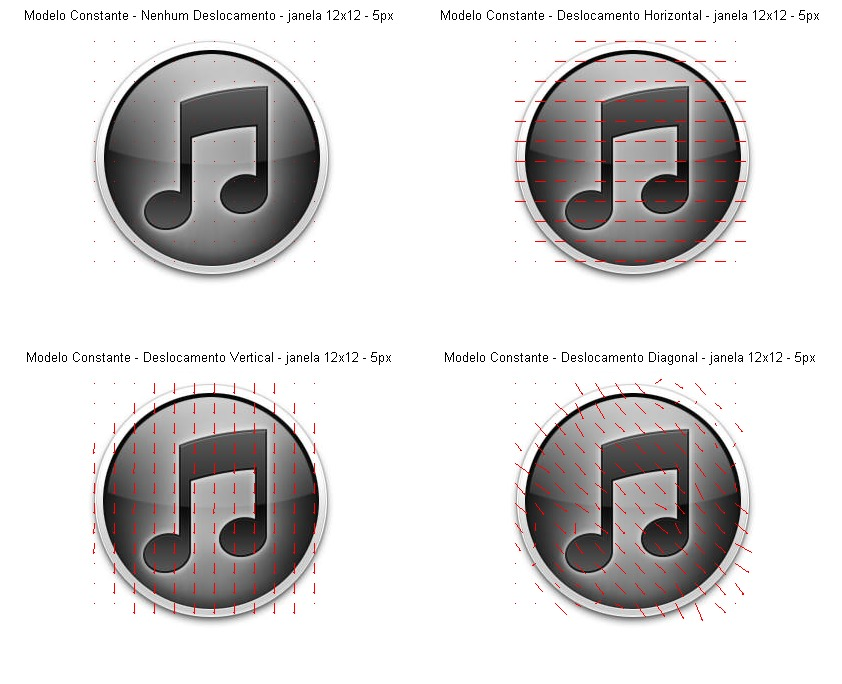
\includegraphics[width=140mm,scale=0.5]{5.jpg}
\caption{Janela de 12x12 - Deslocação de 5 Pixel}\label{fig:5}
\end{figure}

\setlength{\parskip}{20pt}

Comparando a figura \ref{fig:5} com a \ref{fig:3} retiramos a conclusão de que quanto maior a janela escolhida, maior a precisão no cálculo do fluxo óptico. Nesta figura \ref{fig:5} é possivel observar que os vectores de velocidade estão nas direcções correctas como era espectável.
\setlength{\parskip}{10pt}

\textbf{Nota}: Ver valores de $V_x$, $V_y$, $\sigma$ (Modulo e direcção) no \textit{Matlab}.





\newpage

\subsubsection{Modelo Afim - Janela 8x8}



\begin{figure}[ht]
\centering
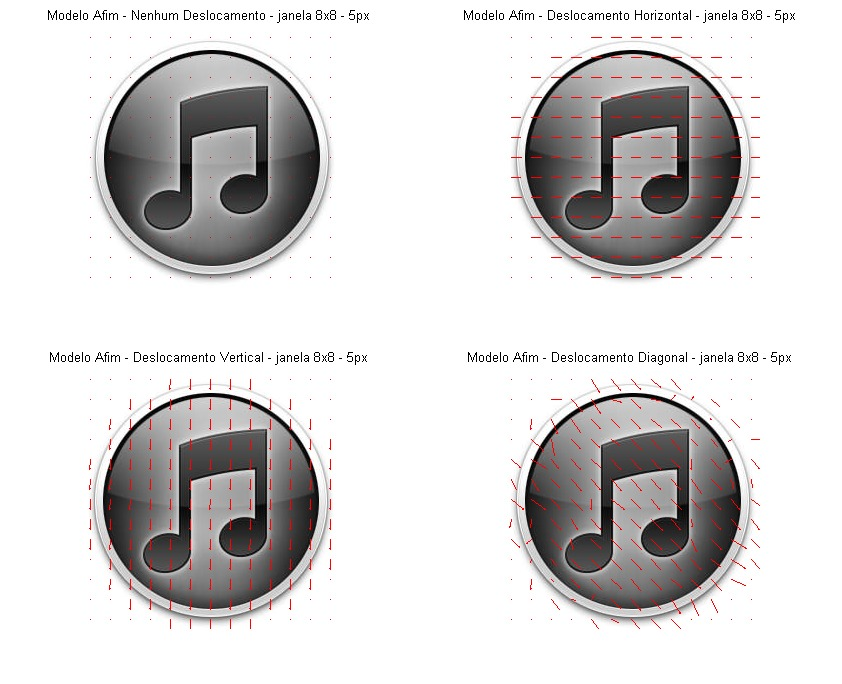
\includegraphics[width=140mm,scale=0.5]{4.jpg}
\caption{Janela de 8x8 - Deslocação de 5 Pixel}\label{fig:4}
\end{figure}


\setlength{\parskip}{20pt}

Na figura \ref{fig:4} retiramos a conclusão de que quanto maior a movimentação dos pixeis pior é o cálculo do fluxo óptico. Este modelo calcula bem os valores do vector de velocidades para movimentações de poucos pixeis, podemos ver por exemplo na deslocação diagonal que os vectores de velocidade não estão todos direcionados na direcção do movimento. 




\newpage

\subsubsection{Modelo Afim - Janela 12x12}



\begin{figure}[ht]
\centering
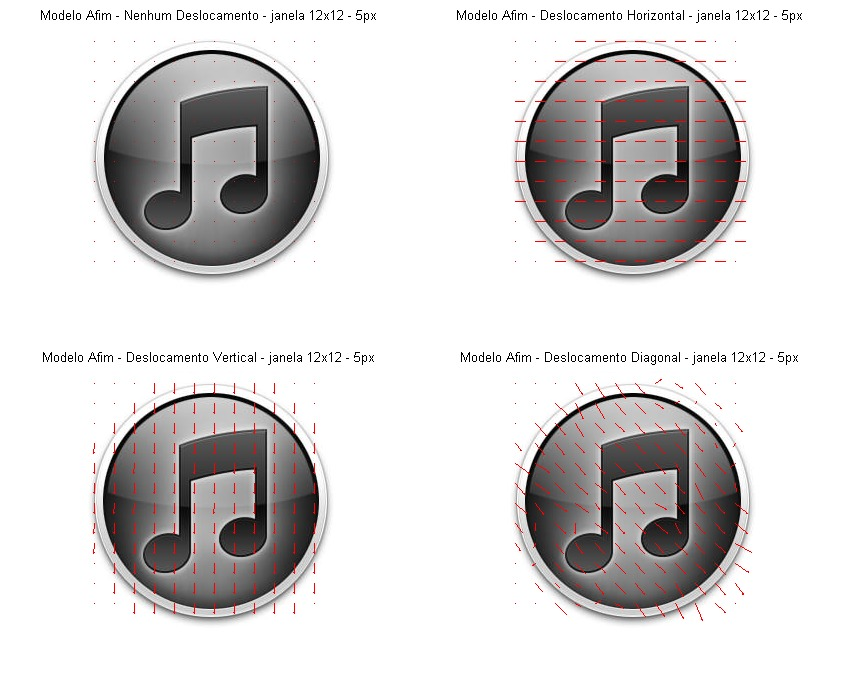
\includegraphics[width=140mm,scale=0.5]{6.jpg}
\caption{Janela de 12x12 - Deslocação de 5 Pixel}\label{fig:6}
\end{figure}


\setlength{\parskip}{20pt}

Comparando a figura \ref{fig:6} com a \ref{fig:4} podemos concluir que ao aumentar o tamanho da janela melhoramos a precisão no cálculo do fluxo óptico como era de se esperar. Além disso, os valores do desvio padrão das imagens correspondentes á figura \ref{fig:6} são menores do que os da figura \ref{fig:4}. Pode-se verificar esta conclusão executando o ficheiro \textit{main} do nosso código.




\newpage




\end{document}
